\documentclass{ximera}

\title{Vraagstukken elektrische krachtwerking: goniometrische figuren}
\author{Daan Lipkens}

\begin{document}
\begin{abstract}
    Oefeningen op coulombkracht met goniometrische figuren.
\end{abstract}
\maketitle

%———————————————————————————————————————
%: OEFENINGEN GONIOMETRISCHE FIGUREN
%———————————————————————————————————————
%\section*{Oefeningen in Goniometrische Figuren}
        
%———————————————————————————————————————
% OEFENING RECHTHOEKIGEDRIEHOEK 1
\begin{exercise}
    Drie puntladingen $Q_{1}= +1{,}5 \cdot 10^{-6} \, \mathrm{C}$, $Q_{2}= +1{,}5 \cdot 10^{-6} \, \mathrm{C}$ en $Q_{3}= -2{,}0 \cdot 10^{-6} \, \mathrm{C}$ bevinden zich in de hoekpunten van een rechthoekige driehoek zoals te zien op de tekening. $Q_{1}$ en $Q_{3}$ liggen $0{,}30 \, \mathrm{m}$ uit elkaar en $Q_{1}$ en $Q_{2}$ liggen $0{,}40 \, \mathrm{m}$ uit elkaar. 
    
    Bereken de grootte van de resulterende kracht op $Q_{3}$.

    \begin{center}
        \begin{tikzpicture}[scale=0.5]
            \useasboundingbox (-1.5, -1.5) rectangle (5.5, 4.5);
            \tkzDefPoint(0,0){A}            
            \begin{scope}[shift=(A)]
                \tkzDefPoint(0:4){B}            
                \tkzDefPoint(90:3){C}       
            \end{scope}
            \tkzDrawPolygon(A,B,C)      
        
            \tkzLabelPoint[left, below=4pt](A){$Q_{1}$}
            \tkzLabelPoint[right, below=4pt](B){$Q_{2}$}
            \tkzLabelPoint[above=4pt](C){$Q_{3}$}
        
            \draw[charge+] (A) circle (\R) node[scale=0.5] {$+$};       
            \draw[charge+] (B) circle (\R) node[scale=0.5] {$+$};
            \draw[charge-] (C) circle (\R) node[scale=0.5] {$-$};
        \end{tikzpicture}
    \end{center}
    
    \[ F_{\text{res},3} = \answer[tolerance=0.05,onlineshowanswerbutton]{0.37} \, \mathrm{N} \]

    \begin{hint}
        Bereken eerst de groottes van de twee afzonderlijke krachten ($F_{13}$ en $F_{23}$) met de wet van Coulomb. Omdat de afstand $r_{23}$ niet gegeven is, moet je deze eerst berekenen met de stelling van Pythagoras in de rechthoekige driehoek.
    \end{hint}
    \begin{hint}
        Teken de krachten in een parallellogram om de resulterende kracht te construeren. Bepaal de hoek in de driehoek bij lading $Q_3$ met behulp van goniometrie ($\tan \theta = \frac{\text{overstaande}}{\text{aanliggende}}$).
    \end{hint}
    \begin{hint}
        Gebruik ten slotte de cosinusregel om de grootte van de resulterende vector te berekenen. Let op: gebruik in de formule van de cosinusregel de \textbf{overstaande hoek} in het krachtenparallellogram!
    \end{hint}

    \begin{solution}\nl
        \underline{Gegevens:}
        \begin{align*}
            & Q_{1} = +1{,}5 \cdot 10^{-6} \, \mathrm{C} & & Q_{2} = +1{,}5 \cdot 10^{-6} \, \mathrm{C} \\
            & Q_{3} = -2{,}0 \cdot 10^{-6} \, \mathrm{C} & & r_{12} = 0{,}40 \, \mathrm{m}\\
            & r_{13} = 0{,}30 \, \mathrm{m} & & 
        \end{align*}

        \underline{Gevraagd:} $ F_{\text{res},3}$\\ 

        \underline{Oplossing:}\\
        Er werken 2 krachten op $Q_{3}$. 
        \begin{itemize}
            \item $F_{13}$ door $Q_{1}$  
            \item $F_{23}$ door $Q_{2}$  
        \end{itemize}
        \textbf{Stap 1: Grootte berekenen}\\ 
        We berekenen de grootte van de deelkrachten.
        \begin{align*}
            F_{13}&=\frac{k\cdot\lvert Q_{1}\rvert\cdot\lvert Q_{3}\rvert}{(r_{13})^{2}} \\
            &=\frac{8{,}99 \cdot 10^9 \, \mathrm{\frac{N \cdot m^2}{C^2}} \cdot 1{,}5 \cdot 10^{-6} \, \mathrm{C} \cdot 2{,}0 \cdot 10^{-6} \, \mathrm{C}}{(0{,}30 \, \mathrm{m})^{2}} \\
            &= 0{,}29966 \, \mathrm{N}
        \end{align*}
        We doen hetzelfde voor $F_{23}$. Hiervoor hebben we eerst $r_{23}$ nodig:
        \begin{align*}
            r_{23} &= \sqrt{r_{12}^{2}+r_{13}^{2}}=\sqrt{(0{,}40 \, \mathrm{m})^{2}+(0{,}30 \, \mathrm{m})^{2}}\\
            &= 0{,}50 \, \mathrm{m}
        \end{align*}
        Zo krijgen we $F_{23}$:
        \begin{align*}
            F_{23}&=\frac{k\cdot\lvert Q_{2}\rvert\cdot\lvert Q_{3}\rvert}{(r_{23})^{2}} \\
            &=\frac{8{,}99 \cdot 10^9 \, \mathrm{\frac{N \cdot m^2}{C^2}} \cdot 1{,}5 \cdot 10^{-6} \, \mathrm{C} \cdot 2{,}0 \cdot 10^{-6} \, \mathrm{C}}{(0{,}50 \, \mathrm{m})^{2}} \\
            &= 0{,}10788 \, \mathrm{N} 
        \end{align*}

        \textbf{Stap 2: Krachten op $Q_{3}$ tekenen}  

        %------------------------------------------------
        % TEKEN DRIEHOEK MET DEELKRACHTEN
        % -----------------------------------------------
        \begin{center}
            \begin{tikzpicture}[scale=0.5]
                \useasboundingbox (-1.5, -1.5) rectangle (5.5, 4.5);
                \tkzDefPoint(0,0){A}            
                \begin{scope}[shift=(A)]
                    \tkzDefPoint(0:4){B}            
                    \tkzDefPoint(90:3){C}       
                \end{scope}
                \tkzDefPointOnLine[pos=2*0.3](C,A)\tkzGetPoint{D} 
                \tkzDefPointOnLine[pos=2*0.17](C,B)\tkzGetPoint{E}  
                \tkzGetPoint{F}             
                \tkzDrawPolygon[dotted, gray](D,C,E,F)      
                \tkzDrawPolygon(A,B,C)      

                % BENOEMEN VAN LADINGEN
                \tkzLabelPoint[left, below=4pt](A){$Q_{1}$}
                \tkzLabelPoint[right, below=4pt](B){$Q_{2}$}
                \tkzLabelPoint[above=4pt](C){$Q_{3}$}

                % LABEL VAN HOEKEN
                \tkzFillAngle[fill=blue!20, opacity=0.5](A,C,B)
                \tkzLabelAngle[pos=1.5](A,C,B){$\theta$}

                % LADING SYMBOOL TEKENEN
                \draw[charge+] (A) circle (\R) node[scale=0.5] {$+$};       
                \draw[charge+] (B) circle (\R) node[scale=0.5] {$+$};
                \draw[charge-] (C) circle (\R) node[scale=0.5] {$-$};
            \end{tikzpicture}
        \end{center}
%----------------------------------------------------------------

    \textbf{Stap 3: Overstaande hoek}\\
        De hoek aan lading $Q_{3}$ kunnen we vinden:
        \begin{align*}
            \tan(\theta)&=\frac{\text{overstaande}}{\text{aanliggende}}\\
            \theta &=\tan^{-1}\left(\frac{0{,}40 \, \mathrm{m}}{0{,}30 \, \mathrm{m}}\right)= 53{,}1^\circ
        \end{align*}
        De hoek tussen $F_{13}$ en $F_{23}$ is dus $53^\circ$. De overstaande hoek van $\vec{\mathbf{F}}_{\text{res}}$ in het parallellogram is $180^\circ - 53{,}1^\circ = 126{,}9^\circ \simeq 127^\circ$.

    \textbf{Stap 4: Cosinusregel gebruiken}  
        \begin{align*}
            F_{\text{res},3} &= \sqrt{F_{13}^{2} + F_{23}^{2} - 2 \cdot F_{13} \cdot F_{23}\cdot \cos(127^\circ)}\\
            &= \sqrt{(0{,}29966 \, \mathrm{N})^{2}+(0{,}10788 \, \mathrm{N})^{2}-2\cdot 0{,}29966 \, \mathrm{N} \cdot 0{,}10788 \, \mathrm{N} \cdot \cos(127^\circ)}\\
            &\simeq 0{,}37 \, \mathrm{N}
        \end{align*}
        De resulterende kracht op lading $Q_{3}$ is ongeveer $3{,}7 \cdot 10^{-1} \, \mathrm{N}$.

    \textbf{Stap 5: Krachten tekenen (optioneel: enkel de grootte is gevraagd.)}

        %------------------------------------------------
        % TEKEN DRIEHOEK MET RESULTERENDE KRACHT
        % -----------------------------------------------
        \begin{center}
            \begin{tikzpicture}[scale=0.8] 
                \useasboundingbox (-1.5, -1.5) rectangle (6, 5);
                \tkzDefPoint(0,0){A}            
                \begin{scope}[shift=(A)]
                    \tkzDefPoint(0:4){B}            
                    \tkzDefPoint(90:3){C}       
                \end{scope}
                \tkzDefPointOnLine[pos=2*0.3](C,A)\tkzGetPoint{D} 
                \tkzDefPointOnLine[pos=2*0.17](C,B)\tkzGetPoint{E}  
                \tkzDrawPoints(D,E)
                \tkzDefParallelogram(D,C,E) 
                \tkzGetPoint{F}             
                \tkzDrawPolygon[dotted, gray](D,C,E,F)      
                \tkzDrawPolygon(A,B,C)      

                % BENOEMEN VAN LADINGEN
                \tkzLabelPoint[left, below=4pt](A){$Q_{1}$}
                \tkzLabelPoint[right, below=4pt](B){$Q_{2}$}
                \tkzLabelPoint[above=4pt](C){$Q_{3}$}


                % LABEL VAN HOEKEN
                \tkzFillAngle[fill=green!20, opacity=0.5](C,E,F)
                \tkzLabelAngle[pos=0.5](C,E,F){$127^\circ$}

                % LADING SYMBOOL TEKENEN
                \draw[charge+] (A) circle (\R) node[scale=1] {$+$};     
                \draw[charge+] (B) circle (\R) node[scale=1] {$+$};
                \draw[charge-] (C) circle (\R) node[scale=1] {$-$};

                % KRACHTEN
                \draw[force] (C)--(D) node[left] {$\vec{\mathbf{F}}_{12}$};
                \draw[force] (C) -- (E) node[above, right] {$\vec{\mathbf{F}}_{13}$};
                \draw[force,red] (C) -- (F) node[right] {$\vec{\mathbf{F}}_{\text{res}}$};
            \end{tikzpicture}
        \end{center}
%----------------------------------------------------------------

    \end{solution}
\end{exercise}
%———————————————————————————————————————

%———————————————————————————————————————
% OEFENING COSINUSREGEL 1: GELIJKZIJDIGEDRIEHOEK
\begin{exercise}
    Drie puntladingen $Q_{1}= +2{,}0 \cdot 10^{-6} \, \mathrm{C}$, $Q_{2}= -3{,}0 \cdot 10^{-6} \, \mathrm{C}$ en $Q_{3}= +4{,}0 \cdot 10^{-6} \, \mathrm{C}$ bevinden zich in de hoekpunten van een gelijkzijdige driehoek met zijde $0{,}50 \, \mathrm{m}$.  

    Bereken de grootte van de resulterende kracht op $Q_{1}$.

    \begin{center}
        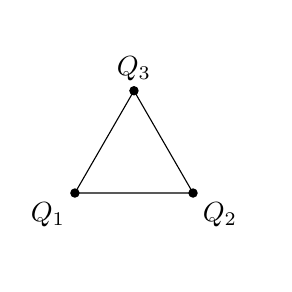
\begin{tikzpicture}[scale=3]
            \useasboundingbox (-0.2, -0.3) rectangle (0.8, 0.7);
            \coordinate (A) at (0,0);
            \coordinate (B) at (0.5,0);
            \coordinate (C) at (0.25,0.433);
        
            \fill (A) circle (0.02) node[below left] {$Q_{1}$};
            \fill (B) circle (0.02) node[below right] {$Q_{2}$};
            \fill (C) circle (0.02) node[above] {$Q_{3}$};
        
            \draw (A) -- (B) -- (C) -- cycle;
        \end{tikzpicture}
    \end{center}
    
    \[ F_{\text{res},1} = \answer[tolerance=0.05,onlineshowanswerbutton]{0.26} \, \mathrm{N} \]

    \begin{hint}
        Bereken eerst $F_{21}$ en $F_{31}$. Welke krachten zijn aantrekkend en welke zijn afstotend? (Lading 2 is negatief en lading 3 is positief).
    \end{hint}
    \begin{hint}
        Omdat het een gelijkzijdige driehoek is, zijn alle inwendige hoeken gelijk aan $60^\circ$. Bepaal door het tekenen van de twee krachtvectoren de hoek tussen de vectoren. Let op: het is niet zomaar $60^\circ$!
    \end{hint}

    \begin{solution}\nl
        \underline{Gegevens:}
        \begin{align*}
            & Q_{1} = +2{,}0 \cdot 10^{-6} \, \mathrm{C} & & Q_{2} = -3{,}0 \cdot 10^{-6} \, \mathrm{C}\\
            & Q_{3} = +4{,}0 \cdot 10^{-6} \, \mathrm{C} & & r_{12}=r_{23}=r_{13}=r = 0{,}50 \, \mathrm{m}
        \end{align*}

        \underline{Gevraagd:} $\vec{F}_{res}$ op $Q_{1}$ \\

        \underline{Oplossing:}\\
        Krachten op $Q_{1}$:  
        \begin{itemize}
            \item $F_{21}$ door $Q_{2}$  
            \item $F_{31}$ door $Q_{3}$  
        \end{itemize}

        \textbf{Stap 1: Grootte berekenen}  
        \[
            F_{12} = \frac{k \cdot \lvert Q_{1}\rvert \cdot\lvert Q_{2}\rvert}{r^{2}} = 
            \frac{8{,}99 \cdot 10^9 \, \mathrm{\frac{N \cdot m^2}{C^2}} \cdot 2{,}0 \cdot 10^{-6} \, \mathrm{C} \cdot 3{,}0 \cdot 10^{-6} \, \mathrm{C}}{(0{,}50 \, \mathrm{m})^{2}} 
            = 0{,}21576 \, \mathrm{N}
        \]
        \[
            F_{13} = \frac{k \cdot \lvert Q_{1}\rvert \cdot \lvert Q_{3}\rvert}{r^{2}} = 
            \frac{8{,}99 \cdot 10^9 \, \mathrm{\frac{N \cdot m^2}{C^2}} \cdot 2{,}0 \cdot 10^{-6} \, \mathrm{C} \cdot 4{,}0 \cdot 10^{-6} \, \mathrm{C}}{(0{,}50 \, \mathrm{m})^{2}} 
            = 0{,}28768 \, \mathrm{N}
        \]

        \textbf{Stap 2: Overstaande hoek}  
        In een gelijkzijdige driehoek zijn de hoeken gelijk aan $60^\circ$. Omdat $Q_2$ aantrekt en $Q_3$ afstoot, is de hoek tussen de vectoren $F_{21}$ en $F_{31}$ gelijk aan $120^\circ$. De overstaande hoek in het parallellogram voor $\vec{\mathbf{F}}_{\text{res}}$ is $60^\circ$.
        \begin{hint}
            Hoeken parallelogram:
                \begin{align*}
                    &360^\circ=2\cdot\alpha+2\cdot\beta\\
                    &\Rightarrow \alpha = \beta - 180^\circ
                \end{align*}
        \end{hint}
        \textbf{Stap 3: Cosinusregel gebruiken}  
        \begin{align*}
            F_{\text{res},1} &= \sqrt{F_{21}^{2} + F_{31}^{2} - 2 \cdot F_{12} \cdot F_{13}\cdot \cos(60^\circ)}\\
            &= \sqrt{(0{,}21576 \, \mathrm{N})^{2}+(0{,}28768 \, \mathrm{N})^{2}-2\cdot 0{,}21576 \, \mathrm{N} \cdot 0{,}28768 \, \mathrm{N} \cdot \cos(60^\circ)}\\
            &\simeq 0{,}26 \, \mathrm{N}
        \end{align*}
        De resulterende kracht op $Q_{1}$ bedraagt dus ongeveer $2{,}6 \cdot 10^{-1} \, \mathrm{N}$.
    \end{solution}
\end{exercise}
%———————————————————————————————————————



%———————————————————————————————————————
% OEFENING EXTRA 1: Rechthoekige driehoek (Pythagoras)
\begin{exercise}
    Drie puntladingen bevinden zich in een assenstelsel. Lading $Q_{1} = -5{,}0 \cdot 10^{-6} \, \mathrm{C}$ ligt in de oorsprong $(0{,}00 \, \mathrm{m} ; 0{,}00 \, \mathrm{m})$. Lading $Q_{2} = +4{,}0 \cdot 10^{-6} \, \mathrm{C}$ ligt op de $x$-as op een afstand van $0{,}40 \, \mathrm{m}$ van de oorsprong. Lading $Q_{3} = +3{,}0 \cdot 10^{-6} \, \mathrm{C}$ ligt op de $y$-as op een afstand van $0{,}30 \, \mathrm{m}$ van de oorsprong.

    Bereken de grootte van de resulterende netto kracht op $Q_{1}$.

    \begin{center}
        \begin{tikzpicture}[scale=1]
            \useasboundingbox (-1.5, -1.5) rectangle (5.5, 4.5);
            \coordinate (A) at (0,0);
            \coordinate (B) at (4,0);
            \coordinate (C) at (0,3);
            
            % Driehoek en assen tekenen
            \draw[dashed, gray] (A) -- (B) node[midway,below] {$0{,}40 \, \mathrm{m}$};
            \draw[dashed, gray] (A) -- (C) node[midway,left] {$0{,}30 \, \mathrm{m}$};
            \draw[dashed, lightgray] (C) -- (B);
        
            % Ladingen labelen
            \tkzLabelPoint[below left](A){$Q_{1}$}
            \tkzLabelPoint[below right](B){$Q_{2}$}
            \tkzLabelPoint[above left](C){$Q_{3}$}
        
            % Ladingen tekenen
            \draw[charge-] (A) circle (\R) node[scale=1] {$-$};       
            \draw[charge+] (B) circle (\R) node[scale=1] {$+$};
            \draw[charge+] (C) circle (\R) node[scale=1] {$+$};
        \end{tikzpicture}
    \end{center}
    
    \[ F_{\text{res},1} = \answer[tolerance=0.05,onlineshowanswerbutton]{1.87} \, \mathrm{N} \]

    \begin{hint}
        Teken eerst de krachten $\vec{\mathbf{F}}_{21}$ en $\vec{\mathbf{F}}_{31}$. Omdat $Q_1$ negatief is en de andere twee positief zijn, zijn het beide aantrekkingskrachten.
    \end{hint}
    \begin{hint}
        Bereken de groottes van $F_{21}$ en $F_{31}$ met de wet van Coulomb. Omdat de ladingen op de $x$- en $y$-as liggen, staan de vectoren perfect loodrecht ($90^\circ$) op elkaar.
    \end{hint}
    \begin{hint}
        Als de hoek tussen twee vectoren $90^\circ$ is, vereenvoudigt de cosinusregel zich tot de stelling van Pythagoras: $F_{\text{res}} = \sqrt{F_{21}^2 + F_{31}^2}$.
    \end{hint}

    \begin{solution}\nl
        \underline{Gegevens:}
        \begin{align*}
            & Q_{1} = -5{,}0 \cdot 10^{-6} \, \mathrm{C} & & \\
            & Q_{2} = +4{,}0 \cdot 10^{-6} \, \mathrm{C} & & r_{12} = 0{,}40 \, \mathrm{m}\\
            & Q_{3} = +3{,}0 \cdot 10^{-6} \, \mathrm{C} & & r_{13} = 0{,}30 \, \mathrm{m}
        \end{align*}

        \underline{Gevraagd:} $F_{\text{res},1}$\\ 

        \underline{Oplossing:}\\
        We berekenen eerst de groottes van de twee krachten die inwerken op lading $Q_{1}$.
        \begin{align*}
            F_{21} &= k\frac{\lvert Q_{2}\rvert\cdot\lvert Q_{1}\rvert}{(r_{12})^{2}} \\
            &= \frac{8{,}99 \cdot 10^9 \, \mathrm{\frac{N \cdot m^2}{C^2}} \cdot 4{,}0 \cdot 10^{-6} \, \mathrm{C} \cdot 5{,}0 \cdot 10^{-6} \, \mathrm{C}}{(0{,}40 \, \mathrm{m})^{2}} \\
            &= 1{,}1238 \, \mathrm{N}
        \end{align*}
        Deze kracht is een aantrekking en wijst dus langs de $x$-as naar rechts.
        
        \begin{align*}
            F_{31} &= k\frac{\lvert Q_{3}\rvert\cdot\lvert Q_{1}\rvert}{(r_{13})^{2}} \\
            &= \frac{8{,}99 \cdot 10^9 \, \mathrm{\frac{N \cdot m^2}{C^2}} \cdot 3{,}0 \cdot 10^{-6} \, \mathrm{C} \cdot 5{,}0 \cdot 10^{-6} \, \mathrm{C}}{(0{,}30 \, \mathrm{m})^{2}} \\
            &= 1{,}4983 \, \mathrm{N}
        \end{align*}
        Deze kracht is eveneens een aantrekking en wijst dus langs de $y$-as naar boven.

        Omdat de vectoren op de assen liggen, is de hoek hiertussen exact $90^\circ$. We kunnen de grootte van de resulterende vector daarom eenvoudig met de stelling van Pythagoras berekenen:
        \begin{align*}
            F_{\text{res},1} &= \sqrt{F_{21}^{2} + F_{31}^{2}} \\
            &= \sqrt{(1{,}1238 \, \mathrm{N})^{2} + (1{,}4983 \, \mathrm{N})^{2}} \\
            &= \sqrt{1{,}2628 + 2{,}2450} \\
            &= \sqrt{3{,}5078} \\
            &= 1{,}8729 \, \mathrm{N} \simeq 1{,}9 \, \mathrm{N}
        \end{align*}
        De resulterende kracht is ongeveer $1{,}9 \, \mathrm{N}$ groot.
    \end{solution}
\end{exercise}
%———————————————————————————————————————

%———————————————————————————————————————
% OEFENING EXTRA 2: Vierkant (Complexe Vectoriële Optelling)
\begin{exercise}
    Vier puntladingen bevinden zich op de hoekpunten van een vierkant met zijde $0{,}20 \, \mathrm{m}$.  
    Lading $Q_{1} = +2{,}0 \cdot 10^{-6} \, \mathrm{C}$ bevindt zich linksonder. Lading $Q_{2} = -2{,}0 \cdot 10^{-6} \, \mathrm{C}$ bevindt zich rechtsonder. Lading $Q_{3} = +2{,}0 \cdot 10^{-6} \, \mathrm{C}$ bevindt zich rechtsboven. Lading $Q_{4} = -2{,}0 \cdot 10^{-6} \, \mathrm{C}$ bevindt zich linksboven.
    
    \begin{question}
        Maak eerst een snelle tekening van de drie afzonderlijke krachten die op $Q_{1}$ inwerken ($\vec{\mathbf{F}}_{21}$, $\vec{\mathbf{F}}_{31}$ en $\vec{\mathbf{F}}_{41}$). Hoe liggen deze drie krachten ten opzichte van elkaar?
        
        \begin{multipleChoice}
            \choice{Ze wijzen alle drie naar rechtsboven.}
            \choice[correct]{Twee krachten staan loodrecht op elkaar, de derde ligt exact op dezelfde as (diagonaal) als hun resulterende kracht.}
            \choice{Ze heffen elkaar perfect op tot een netto kracht van 0 N.}
        \end{multipleChoice}
        
        \begin{hint}
            $Q_2$ en $Q_4$ zijn negatief, dus zij trekken het positieve $Q_1$ aan. Dit vormt twee loodrechte krachten (langs de zijden van het vierkant). $Q_3$ is óók positief, dus die stoot $Q_1$ af. Die kracht ligt op de verlengde diagonaal van het vierkant!
        \end{hint}
    \end{question}
    
    \begin{question}
        Bereken nu de grootte van de totale resulterende kracht op $Q_{1}$.
        
        \[ F_{\text{res},1} = \answer[tolerance=0.05,onlineshowanswerbutton]{0.82} \, \mathrm{N} \]

        \begin{hint}
            Stap 1: Bereken $F_{21}$ en $F_{41}$ met de wet van Coulomb. Omdat ze loodrecht op elkaar staan, kan je hiervan eenvoudig een eerste resultante $\vec{\mathbf{F}}_{24}$ berekenen met Pythagoras.
        \end{hint}
        \begin{hint}
            Stap 2: Bereken $F_{31}$. Let op: de afstand tot $Q_3$ is de diagonaal van het vierkant. Deze diagonaal bereken je met Pythagoras: $r_{13} = \sqrt{(0{,}20)^2 + (0{,}20)^2}$.
        \end{hint}
        \begin{hint}
            Stap 3: $\vec{\mathbf{F}}_{24}$ trekt $Q_1$ naar het midden van het vierkant. $\vec{\mathbf{F}}_{31}$ duwt $Q_1$ weg van het midden (afstoting). Omdat deze vectoren op perfect dezelfde as (de diagonaal) liggen, mag je ze wiskundig gewoon van elkaar aftrekken!
        \end{hint}

        \begin{solution}\nl
            \underline{Gegevens:}
            \begin{align*}
                & \lvert Q_{1} \rvert = \lvert Q_{2} \rvert = \lvert Q_{3} \rvert = \lvert Q_{4} \rvert = 2{,}0 \cdot 10^{-6} \, \mathrm{C} \\
                & r_{12} = r_{14} = 0{,}20 \, \mathrm{m}
            \end{align*}
    
            \underline{Gevraagd:} $F_{\text{res},1}$\\ 
    
            \underline{Oplossing:}\\
            Er werken drie krachten op $Q_1$. We rekenen ze in stappen uit.
            
            \textbf{Stap 1: De krachten langs de randen}\\
            De ladingen $Q_2$ en $Q_4$ zijn negatief. Zij trekken het positieve $Q_1$ aan met krachten $\vec{\mathbf{F}}_{21}$ en $\vec{\mathbf{F}}_{41}$. Omdat afstanden en ladingen identiek zijn, zijn deze krachten even groot:
            \[
                F_{21} = F_{41} = \frac{8{,}99 \cdot 10^9 \cdot (2{,}0 \cdot 10^{-6}) \cdot (2{,}0 \cdot 10^{-6})}{(0{,}20)^2} = 0{,}899 \, \mathrm{N}
            \]
            We bundelen deze twee loodrechte vectoren met de stelling van Pythagoras tot één resulterende 'trekkracht' ($\vec{\mathbf{F}}_{24}$) in de richting van het midden van het vierkant:
            \[
                F_{24} = \sqrt{(0{,}899)^2 + (0{,}899)^2} = \sqrt{2} \cdot 0{,}899 \simeq 1{,}271 \, \mathrm{N}
            \]
            
            \textbf{Stap 2: De afstotende diagonale kracht}\\
            Lading $Q_3$ bevindt zich op de diagonaal. We berekenen eerst de afstand $r_{13}$ (de lengte van de diagonaal):
            \[
                r_{13} = \sqrt{(0{,}20)^2 + (0{,}20)^2} = \sqrt{0{,}08} \simeq 0{,}2828 \, \mathrm{m}
            \]
            Beide ladingen zijn positief, dus $Q_3$ stoot $Q_1$ af, weg van het centrum van het vierkant:
            \[
                F_{31} = \frac{8{,}99 \cdot 10^9 \cdot (2{,}0 \cdot 10^{-6}) \cdot (2{,}0 \cdot 10^{-6})}{(\sqrt{0{,}08})^2} = \frac{0{,}03596}{0{,}08} = 0{,}4495 \, \mathrm{N}
            \]

            \textbf{Stap 3: Alles samenbrengen}\\
            De aantrekkingskracht $F_{24}$ wijst via de diagonaal \emph{naar het midden}.
            De afstotingskracht $F_{31}$ wijst langs exact dezelfde as \emph{van het midden weg}.
            Omdat ze een tegengestelde zin hebben op dezelfde lijn, mogen we ze simpelweg aftrekken:
            \[
                F_{\text{res}} = F_{24} - F_{31} = 1{,}271 \, \mathrm{N} - 0{,}4495 \, \mathrm{N} = 0{,}8215 \, \mathrm{N} \simeq 8{,}2 \cdot 10^{-1} \, \mathrm{N}
            \]
            De netto kracht trekt lading $Q_1$ schuin naar het centrum van het vierkant.
        \end{solution}
    \end{question}
\end{exercise}
%———————————————————————————————————————

\end{document}